% ══════════════════════════════════════════════════════════════════
\chapter{Can We Fix the Kernel Instead of the Weights?}
\label{ch:kernel}
% ══════════════════════════════════════════════════════════════════

The previous chapters showed that constraining the weights (row
centering) kills the forward signal.  This chapter explores two
alternative approaches: modifying the ReLU nonlinearity via a negative
bias, and analyzing the solutions found by direct kernel optimization.

% ──────────────────────────────────────────────────────────────────
\section{Biased ReLU Kernel $K_\beta(\alpha)$}
\label{sec:biased_relu}

\subsection{Motivation}

Instead of constraining~$W$, add a negative bias $b < 0$ to raise
the ReLU threshold: $\relu(z + b)$ fires only when $z > -b > 0$.
This kills weakly-positive activations (which contribute to DC drift)
while keeping the weight matrix \textbf{unconstrained} --- no
zero-sum rows, so no gradient trap from the weight structure.

\subsection{Definition}

Let $(\bm{x}_i, \bm{x}_j)$ be unit vectors with angle $\alpha$.
For a weight vector $\bm{w} \sim \mathcal{N}(\bm{0}, \sigma^2 I)$
and normalized bias $\beta = b/\sigma$, the biased kernel is:
\begin{equation}\label{eq:biased_kernel}
  K_\beta(\alpha)
  = \E\!\bigl[\relu(u + \beta) \cdot \relu(v + \beta)\bigr],
\end{equation}
where $(u,v) \sim \mathcal{N}\!\bigl(\bm{0},
\bigl[\begin{smallmatrix} 1 & \cos\alpha \\
\cos\alpha & 1\end{smallmatrix}\bigr]\bigr)$.

At $\beta = 0$, this reduces to the standard arc-cosine kernel
(Theorem~\ref{thm:kernel} with $\sigma = 1$).

\subsection{Optimization objective}

Define the normalized distortion:
\begin{equation}
  D_\beta(\alpha)
  = \frac{K_\beta(\alpha)}{K_\beta(0)} - \cos\alpha.
\end{equation}
We seek $\beta^*$ minimizing the integrated squared distortion:
\begin{equation}
  \beta^*
  = \argmin_{\beta \leq 0}
    \int_0^{\pi} D_\beta(\alpha)^2 \, d\alpha.
\end{equation}

\subsection{Monte Carlo evaluation}

Since there is no known closed-form for $K_\beta(\alpha)$ when
$\beta \neq 0$, we evaluate it via Monte Carlo with $10^6$ samples.
At $\beta = 0$, the MC estimate matches the analytical $K(\alpha)$
to within 1.3\% relative error, confirming sufficient accuracy.

\begin{figure}[h]
\centering
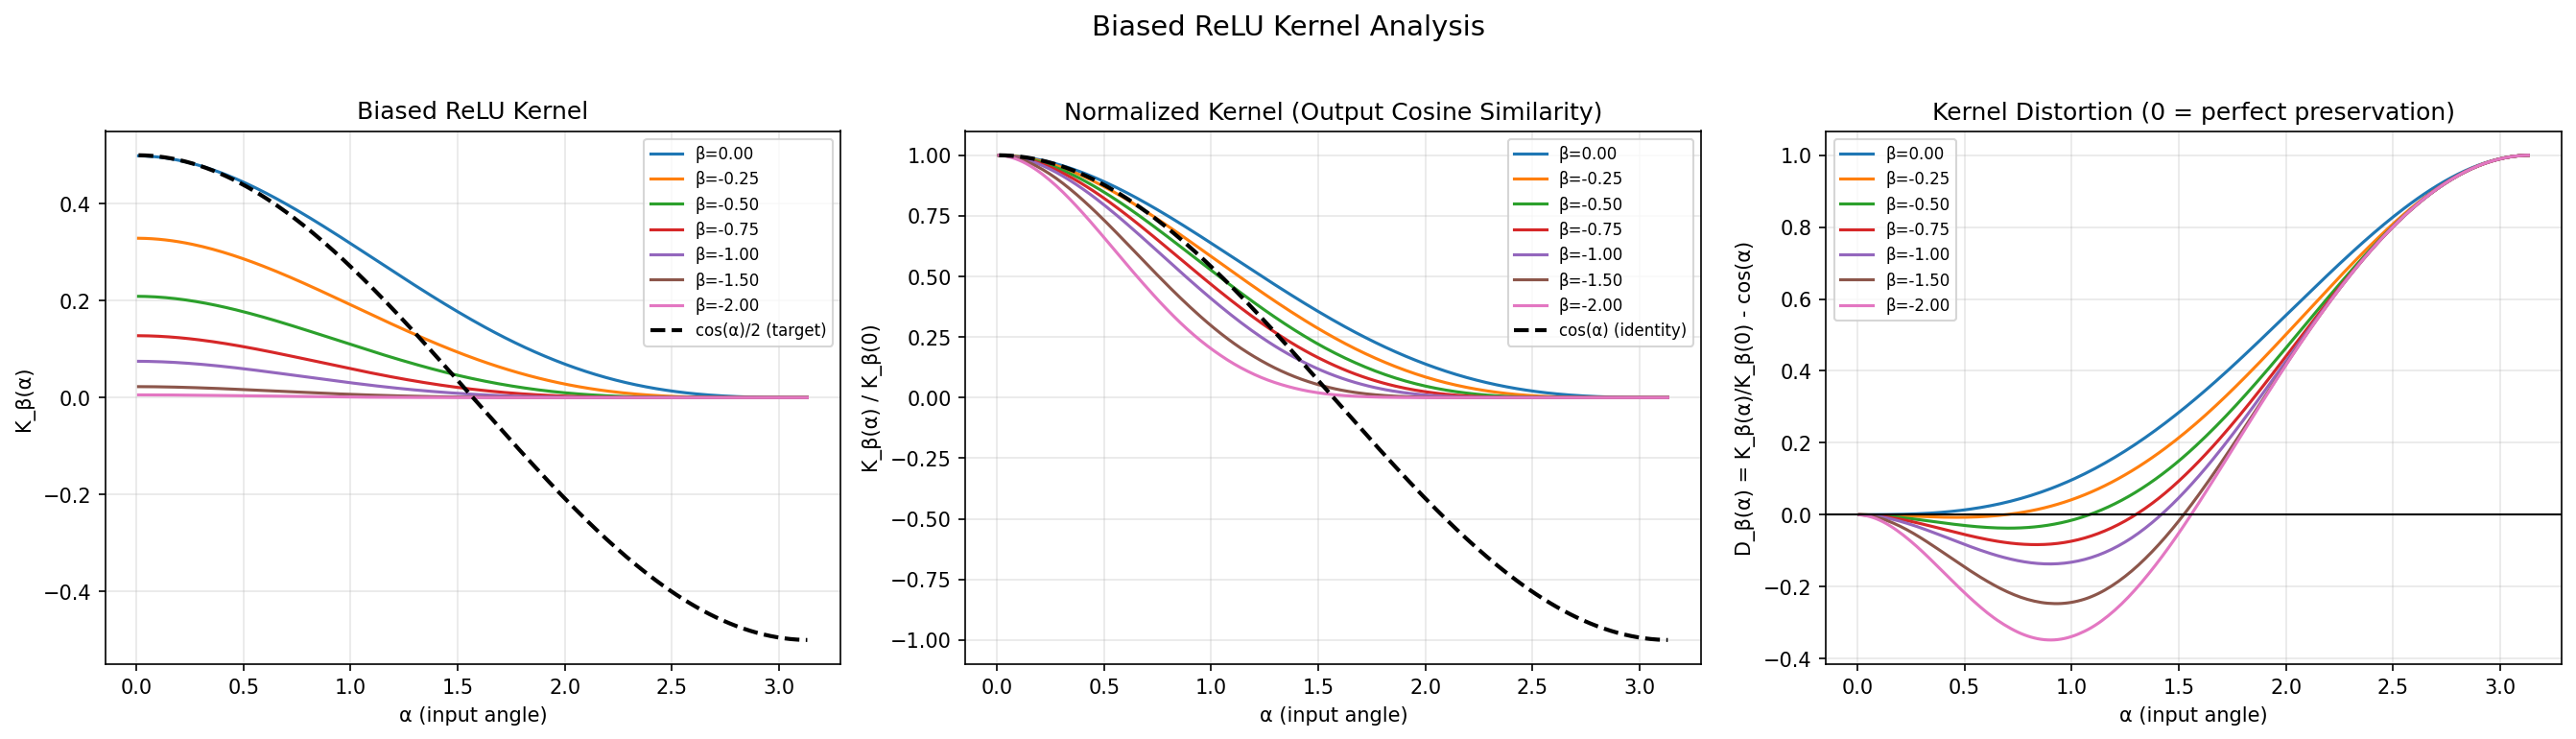
\includegraphics[width=\textwidth]{figures/biased_relu_kernel.png}
\caption{Biased ReLU kernel analysis.
  \textbf{Left:} Raw kernel $K_\beta(\alpha)$ for various $\beta$.
  \textbf{Center:} Normalized kernel (output cosine similarity).
  \textbf{Right:} Kernel distortion $D_\beta(\alpha)$ --- negative bias
  reduces distortion at small angles but overcorrects at large angles.
  Source: \texttt{notebooks/07\_kernel\_geometry\_analysis.ipynb}, Cell~11.}
\label{fig:biased_kernel}
\end{figure}

\subsection{Results}

\begin{center}
\begin{tabular}{cccc}
\toprule
$\beta$ & Integrated distortion & Survival rate $\Phi(\beta)$ &
$\sigma^2_{\mathrm{adj}}$ factor \\
\midrule
$0.00$ & 0.912 & 50.0\% & 1.00 \\
$-0.50$ & 0.843 & 30.9\% & 1.62 \\
$\bm{-0.93}$ & \textbf{0.795} & \textbf{17.6\%} & \textbf{5.72} \\
$-1.50$ & 0.847 & 6.7\% & 14.9 \\
$-2.00$ & 0.905 & 2.3\% & 43.5 \\
\bottomrule
\end{tabular}
\end{center}

\textbf{Optimal bias:} $\beta^* \approx -0.93$.
\textbf{Distortion reduction:} $0.795 / 0.912 = 0.87$, i.e., only a
\textbf{13\% improvement}.

\subsection{Why it doesn't work}

The distortion profiles reveal the mechanism:
\begin{itemize}
  \item For \textbf{small angles} ($\alpha < 1$): negative bias reduces
        distortion (nearby vectors become less artificially similar).
  \item For \textbf{large angles} ($\alpha > 2$): negative bias
        \textbf{overcorrects} --- vectors that were nearly orthogonal
        appear negatively correlated in the output.
  \item No value of $\beta$ reduces distortion uniformly across all
        angles.
\end{itemize}

\subsection{Variance compensation}

At $\beta^* = -0.93$, only 17.6\% of neurons fire, so the output
signal is much weaker.  To maintain the same forward signal strength
as standard He:
\[
  \sigma^2_{\mathrm{adj}}
  = \frac{2/d}{2\,\Phi(\beta^*)} \cdot C(\beta^*)^{-1}
  \approx 5.72 \cdot \frac{2}{d},
\]
where $C(\beta^*)$ is a correction factor from the second moment of
the truncated Gaussian.

This $5.72\times$ variance increase would push the backward gain
well above~1, potentially creating its own gradient instability.

\subsection{Assessment}

Negative bias is a \textbf{dead end}:
\begin{enumerate}
  \item Marginal improvement (13\% distortion reduction) ---
        insufficient to prevent collapse over 20+ layers.
  \item Extreme sparsity (82\% of neurons silent) requiring massive
        variance compensation.
  \item The distortion is reshaped, not eliminated.
  \item \textbf{Fundamental limit:} No pointwise nonlinearity
        (applied independently per neuron) can fully preserve the input
        kernel.  The distortion $D(\alpha)$ is intrinsic to any
        nonlinear map from $\R^2 \to \R$, and a threshold shift can
        only change $D$'s shape, not make it zero everywhere.
\end{enumerate}

% ──────────────────────────────────────────────────────────────────
\section{Analyzing Kernel-Preserving Optimizer Solutions}
\label{sec:kp_analysis}

\subsection{Motivation}

The \texttt{kernel\_preserving} initializer
(Section~\ref{sec:kp_init}) directly minimizes the kernel distortion.
At 5 layers it achieves $k$-NN $= 0.737$ (comparable to He).
By analyzing the structure of the optimized weight matrices, we ask:
\begin{itemize}
  \item Does the optimizer discover row centering?
  \item Does it discover negative bias?
  \item Or something entirely different?
\end{itemize}

We initialize 10 independent layers with \texttt{kernel\_preserving}
and compare the resulting weight matrices to standard He.

\subsection{Results}

\begin{table}[h]
\centering
\begin{tabular}{lccc}
\toprule
Property & He & KP & KP/He ratio \\
\midrule
Mean $|\text{row sum}|$ & 1.2 & 12.2 & $10\times$ \\
Mean row norm $\|\bm{w}_i\|$ & 1.3 & 15.0 & $11.5\times$ \\
Weight distribution & Gaussian & Uniform (flat) & --- \\
Mean pre-activation (DC) & 0.03 & 0.39 & $13\times$ \\
SVD spectrum & Flat ($\sim\!2.5$) & Decaying ($41 \to 20$) & --- \\
\bottomrule
\end{tabular}
\caption{Structural comparison of He vs.\ kernel-preserving weight matrices.}
\label{tab:kp_structure}
\end{table}

\begin{flagbox}
The inner-product and norm terms in the KP objective
\eqref{eq:kp_objective} are normalized by $d_{\mathrm{out}}$.
The norm constraint targets
$\|\relu(W\bm{x})\|^2 / d_{\mathrm{out}} \approx 1$,
which means $\|\relu(W\bm{x})\| \approx \sqrt{d_{\mathrm{out}}}$.
This targeting of output norms $\sqrt{d}$ rather than~$1$ contributes
to the observed $11.5\times$ weight inflation: part of the inflation
is an artifact of this normalization choice.
\end{flagbox}

\subsection{Key findings}

\begin{enumerate}
  \item \textbf{NOT row centering.}
        Row sums are $10\times$ \emph{larger} than He.
        The optimizer moves \textbf{away} from zero row sums.
        If centering were optimal for kernel preservation, the optimizer
        would have converged toward $\sum_j W_{ij} \approx 0$.

  \item \textbf{NOT negative bias.}
        The DC component (mean pre-activation) is $13\times$ larger than He.
        The optimizer \emph{amplifies} the mean, opposite to the biased
        ReLU strategy of Section~\ref{sec:biased_relu}.

  \item \textbf{Uniform, not Gaussian.}
        The weight elements follow a nearly uniform distribution (flat
        histogram, heavy-tailed Q-Q plot vs.\ normal), a radical departure
        from any standard initialization.

  \item \textbf{Anisotropic SVD.}
        The singular value spectrum decays from $\sim\!41$ (top) to
        $\sim\!20$ (bottom), with condition number $\sim\!2\times$
        (vs.\ $\sim\!1.1\times$ for He).
        The optimizer selectively amplifies certain input directions:
        components along top singular vectors get large pre-activations
        and survive ReLU with high probability, while components along
        bottom singular vectors are more likely killed.

  \item \textbf{Massively inflated weights.}
        Row norms $11.5\times$ larger than He.
        This inflation compounds catastrophically at depth:
        $15^L$ grows to astronomical values, causing the float64
        overflow at 20 layers (Section~\ref{sec:kp_failure}).
\end{enumerate}

\subsection{Why the structure is non-composable}

The KP optimizer's anisotropic amplification is tuned to the
\emph{input distribution} (random unit vectors).  After one KP layer
transforms the data, the output distribution is no longer unit vectors
--- it has been selectively amplified and truncated by ReLU.
The next layer's KP optimization, still targeting random unit vectors,
operates under violated assumptions.

Over $L$ layers, the accumulated mismatch between the assumed input
distribution (unit vectors) and the actual input distribution
(increasingly distorted post-ReLU data) causes the optimization to
diverge.

\subsection{Implications}

The optimizer confirms that kernel preservation requires a radically
different weight structure from any standard initialization.
The structure it finds (massive inflation + anisotropy + uniform
weights) is inherently per-layer and data-dependent --- there is no
simple closed-form generalization.

This reinforces the conclusion from Section~\ref{sec:biased_relu}:
the ReLU kernel distortion is a fundamental property of the nonlinearity
that cannot be eliminated by a single-layer weight structure,
regardless of its complexity.
